%%%%%%%%%%%%%%%%%%%%%%%%%%%%%%%%%%%%%%%%%%%%%%%%%%%%%%%%%%%%%%%%%%%%%%%%%%%%%%%%
%2345678901234567890123456789012345678901234567890123456789012345678901234567890
%        1         2         3         4         5         6         7         8

\documentclass[letterpaper, 10 pt, conference]{ieeeconf}  % Comment this line out if you need a4paper
\usepackage{url}
\usepackage{cite}
% The following packages can be found on http:\\www.ctan.org
%\usepackage{graphics} % for pdf, bitmapped graphics files
\usepackage{graphicx} % for pdf, bitmapped graphics files
\usepackage{epsfig} % for postscript graphics files
\usepackage{mathptmx} % assumes new font selection scheme installed
\usepackage{times} % assumes new font selection scheme installed
\usepackage{amsmath} % assumes amsmath package installed
\usepackage{amssymb}  % assumes amsmath package installed
\usepackage{gensymb}
\usepackage{epstopdf}
\usepackage[]{units}
%\usepackage{subscript}
\usepackage{color}
\usepackage{verbatim}
\usepackage{psfrag}
\bibliographystyle{IEEEtran}
\usepackage{textcomp}
\usepackage{graphicx}
%\usepackage{caption}
%\usepackage{subcaption}
%\usepackage{algpseudocode}
\usepackage{algorithmic}
\usepackage[Pseudocode]{algorithm}
%\usepackage{todonotes}
\usepackage{bm}
\usepackage{empheq}
\usepackage{pgfplots}
\usepackage{multirow}
%\usepackage[table,xcdraw]{xcolor}

%% TO USE HYPERREF (BUG IN IEEE style) (REMOVE BEFORE PUBLICATION)
%\makeatletter
%\let\NAT@parse\undefined
%\makeatother
%\usepackage{hyperref}

\pdfminorversion=5
\pgfplotsset{compat=1.13}
%\documentclass[a4paper, 10pt, conference]{ieeeconf}      % Use this line for a4 paper

\IEEEoverridecommandlockouts                              % This command is only needed if 
% you want to use the \thanks command

\overrideIEEEmargins                                      % Needed to meet printer requirements.

% See the \addtolength command later in the file to balance the column lengths
% on the last page of the document

\title{\LARGE \bf
	Dynamic Markers: Optimal control point configurations for homography and pose estimation
}


\author{Raul Acuna$^{1}$ and Volker Willert$^{1}$% <-this % stops a space
	\thanks{*This work was sponsored by the German Academic Exchange Service (DAAD) and the Becas Chile doctoral scholarship.}% <-this % stops a space
	\thanks{$^{1}$These authors are within the Institute of Automatic Control and Mechatronics, Technische Universit{\"a}t Darmstadt, Germany.{\tt\small (racuna, vwillert)}{\tt\small @rmr.tu-darmstadt.de}}}

\begin{document}
	\maketitle
	\thispagestyle{empty}
	\pagestyle{empty}
	%%%%%%%%%%%%%%%%%%%%%%%%%%%%%%%%%%%%%%%%%%%%%%%%%%%%%%%%%%%%%%%%%%%%%%%%%%%%%%%%
	\begin{abstract}
		In this paper, we investigate in the influence of control points on the accuracy of space resection methods, e.g. used by a fiducial marker for pose estimation. More precisely, we propose a gradient descent optimization method to find optimal configurations of control points for the tasks of homography estimation and subsequent planar pose estimation from a number of $n \geq 4$ noisy point correspondences. We obtain optimal configurations by minimizing the first order perturbed solution of the direct linear transformation (DLT) algorithm which is equivalent to minimizing the condition number of the data matrix. This method guarantees point configurations which maximize the robustness of the DLT homography estimation against noise. Furthermore, a statistical evaluation is presented verifying that this optimal control point configurations even increase the performance of very accurate state of the art homography as well as pose estimation methods, like IPPE and EPnP, including the iterative minimization of the reprojection error MRE which is the most accurate algorithm. Finally, we provide a tradeoff between optimal configuration and the number of control points.
	\end{abstract}
	
	%(3D-2D)
	%(that minimize the sensitivity to noise)
	%(condition number of the data matrix in the)
	%(for the minimal number of four control points sets (also 5 and 6?) found)
	%These results shed some light on the influence of the control model points on the accuracy %of space resectioning methods, which has been an open problem in the literature so far.
	%(not only for the DLT transform but as well for other homography estimation methods).
	%(Finally, looking at the statistics of the point configurations, we derive new rotation and %scaling invariant coordinate normalizations $T(H)$ as a function of the homography itself.
	
	%%%%%%%%%%%%%%%%%%%%%%%%%%%%%%%%%%%%%%%%%%%%%%%%%%%%%%%%%%%%%%%%%%%%%%%%%%%%%%%%
	\section{INTRODUCTION}
	%Why?
	The Perspective-n-Point (PnP) problem also known as space resection and the special case of planar pose estimation via homography estimation are some of the most researched topics in the fields of computer vision and photogrammetry. Even though the research in these areas has been wide, there is a surprising lack of information regarding the effect of the 3D control point configurations on the accuracy and robustness of the estimation methods.
	
	%What? For Whom?
	As will be shown in Sec.~\ref{state_of_the_art}, it is clear from the literature, that the control point configurations are relevant and do influence accuracy as well as robustness of the pose estimates. 
	However, these findings are rather general because they are based on hands-on experience and thus far only lead to some rules of thumb. Most obvious and widely accepted is, that increasing the number of control points increases the accuracy of the results in presence of noise. Further on, in several studies when simulations are performed to compare methods, great care is given to possible singular point configurations, such as non-centered data or near-planar cases which are singularities or degenerate cases for certain estimation methods. 
	
	A more thorough evaluation is given for the \textit{normalized} DLT algorithm, whereas the normalization has already shown to improve the estimation because it is related to the condition number of the set of DLT equations \cite{Hartley1997}. The only error analysis for homography estimation found so far by the authors in the literature presents a statistical analysis and simulations of the errors in the homography coefficients \cite{Chen2009}.
	
	\begin{figure}[t]
		\begin{center}
			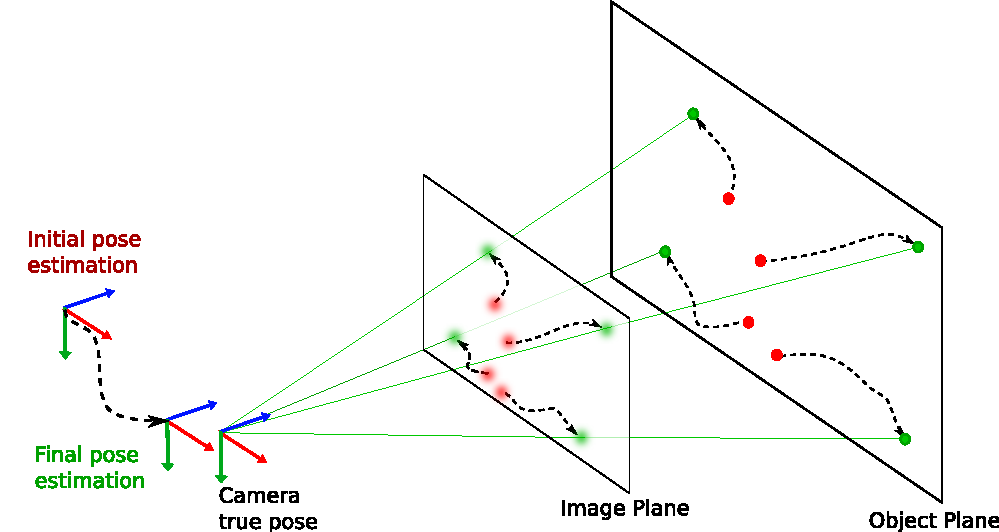
\includegraphics[width=\columnwidth]{img/intro_figure.pdf}
			\caption{\label{fig:intro_figure}\small The idea of a dynamic marker: The control points with known 3D coordinates on the object plane (marker) in arbitrary configuration (red) are moved towards optimal configurations (green) for pose estimation from these control points and their corresponding noisy projections on the image plane (blurry red and green). The control points' dynamics \eqref{Eq12} is given by the gradient descent steps minimizing the optimization objective \eqref{Eq11} that results in optimal pose estimations (from red to green) close to the true camera pose (black).}
		\end{center}
		\vspace{-0.7cm}
	\end{figure}
	
	However, none of the above give an answer to the question: 
	\textit{Is there an optimal perspective-n-point configuration, which can increase the accuracy and robustness of space resection methods?}
	
	If there is an optimal configuration, this question includes several follow-up questions: 
	Is this optimal configuration dependent on the pose, or is there only one configuration that is optimal for all poses? What are the specifics of this/these configuration(s) in relation to absolute coordinates and relative distances between coordinates? Are there similarities between configurations that differ in the number of control points? When does an increase in number of points that are arbitrarily configured outperform the optimal configuration of a small number point set?  
	
	In this paper, we give an answer to all of these questions for planar control points by proposing an optimization objective to find optimal planar control point configurations. Figure~\ref{fig:intro_figure} sketches the main idea of optimizing the proposed objective via a gradient descent approach and the stepwise improvement of the accuracy of the pose estimate starting from some initial control point configuration. Each descent step leads to a change in control point configuration and thus defines a dynamics for the control points that are placed on a planar visual fiducial marker (object plane), which we call a \textit{dynamic marker}.
	This research could be relevant both for those interested on the development of algorithms for PnP and space resection, as well for the community of fiducial marker designers.
	
	%	Many more questions are also connected to this main one:
	%	
	%	\begin{itemize}
	%		\item May a well conditioned n-points configuration be better than a (an ill-conditioned or) %random configuration with more points? 
	%		\item A wider separation between points is better?
	%		\item Is there a configuration which is better for all camera poses, or on the other hand there %is a best point configuration for each pose? Is the optimal point configuration dependent on the %homography/camera pose itself?
	%		\item If there is an optimal configuration, is it invariant to the intrinsic camera parameters?
	%	\end{itemize}
	
	
	
	%In absence of noise the PnP methods and homography estimation methods return the true solution. The problem is the image and model noise propagation in the pose estimation process. If it were possible to select the control points it would be obvious to select those which increase the robustness of the algorithms in presence of noise. It is relevant that even with the great amount of research in this field there is not much information about the influence of the control point configurations and no clear answer to the best possible point configuration is given besides the vague suggestions and classifications presented above. 
	
	%In this paper we propose a simple approach to find optimal control points configurations. We assume that there must exist a metric which represents the robustness of a given point configuration to noise for homography estimation and PnP methods. The problem is then to find a suitable metric and then use it as cost function which has to be minimized by moving the control points in the space. The location of the minima for a given number of points should be the one that increases the robustness of the estimation methods versus noise.
	
	%	The goal of the present work is to define a method that can be used to obtain optimal control points configuration that increase the robustness of the homography estimation and a possible subsequent pose estimation in the presence of noise. 
	
	%We propose the use of a gradient search approach to move the control points in space in order to find the minimum of an optimality condition. The homography was selected as a simple basis for space resectioning, thus restricting the control points configurations to a plane. The optimality condition was defined as the condition number of the $A$ matrix in the DLT method of homography estimation, since it improves the stability of the SVD decomposition and its robustness to noise as it will be described in Chapter \ref{XXXXX}.
	
	
	
	%It will be possible to predict the robustness of a given set of control points by only finding the condition number of their associated A matrix.
	
	%Some questions:
	
	%It is usually recommended when estimating homographies to select control points as widely separated as possible, is this true? does it really give better results?. 
	
	%It is known as well that increasing the amount of points increases the robustness of the estimation to noise. Is it possible that a well conditioned 4 point configuration may be better than ill conditioned or random configurations with more points?.
	
	%Are there any point configurations which can be on average more robust to noise than others? if so, how can this configuration be found?
	
	%Is there a preferred configuration which is better for all camera poses, or on the other hand the best point configuration is pose dependent?
	%Is it invariant to camera parameters?
	
	%When testing and comparing PnP or homography estimation algorithms usually a set of random points or a a selection of evenly distributed points within some limits are selected, there is no standard guideline for the selection of this points. It may be interesting to have a basic configuration, robust to noise for all the methods, that can facilitate the comparison and which can avoid the presence of local minima or singularities in the solutions.
	
	%A thorough analysis of the state of the art in homography and pose estimation methods was performed in search for suggestions about the optimality of the control points configuration, the results of this search are presented at the end of the state of the art chapter TODO with a summary of the vague information that we could trace in the literature.
	% \begin{figure}[htb]
	%      \centering
	%       \includegraphics[draft,width=0.5\textwidth]{Interesting-Image-for-the-reader.png}
	%       \caption{A}\label{A}
	% \end{figure}
	
	The paper is structured as follows:  In Sec.~\ref{state_of_the_art}, we classify pose estimation methods and summarize known findings about control point configurations. In Sec.~\ref{SecBasics}, we derive the optimization objective based on golden standard algorithms for pose estimation. In Sec.~\ref{SimSetup}, we describe the simulation results, and finally in Sec.~\ref{Conc}, we discuss the results and give conclusions.
	
	\section{state of the art}
	\label{state_of_the_art}
	\subsection{Brief history of space resection and PnP methods}
	Camera or space resection is a term used in the field of photogrammetry in which the spatial position and orientation of a photo is obtained by using image measurements of control points present on the photo. A similar concept comes from the computer vision community, where it is known as the Perspective-n-Point (PnP) problem. PnP can be considered an over-constrained (only for $n \geq 3$) and generic solution to the pose estimation problem from point correspondences. PnP methods can be classified into those which solve for a small and predefined number $n$ of points, and those which can handle the general case. The minimal number of points to solve the PnP problem is three. Several solutions have been presented in the literature~\cite{Marchand2016}, which in general provide four solutions for non-collinear points. Thus, prior knowledge has to be included to choose the correct solution. 
	
	%We look at the number of constraints in terms of 	corresponding features required to estimate the 	projective transformation H.  A lower bound 	is available from the number of degrees 	of freedom and the number of constraints. 	The matrix H contains 9 entries, but 	is defined only up to scale. 	Thus, the total number of degrees of freedom 	in a 2D projective transformation is 8. 	Each corresponding 2D point or line 	generates two constraints on H 	by Equation $x' = Hx$ and hence 	the correspondence of four points 	or four lines is sufficient to compute H (A Survey of Planar 	Homography Estimation Techniques, 2009). 
	
	Since it has been proven that pose accuracy usually increases with the number of points \cite{Marchand2016}, other PnP approaches that use more points ($n > 3$) are usually preferred. The general PnP methods can be broadly divided into whether they are iterative or non-iterative. Iterative approaches formulate the problem as a non-linear least-squares problem. They differ in the choice of the cost function to minimize, which is usually associated to an algebraic or geometric error. Some of the most important iterative methods in chronological order are: the \textbf{POSIT} algorithm~\cite{Oberkampf1996}, the \textbf{LHM}~\cite{Lu2000}, the Procrustes PnP method or \textbf{PPnP}~\cite{Garro2012} and the global optimization method \textbf{SDP}~\cite{Schweighofer2008}.
	
	%%%%%%%%%%%%%%%%%%%%%%%%%%%%
	%The \textbf{POSIT} algorithm~\cite{Oberkampf1996} is one of the first iterative solutions. It consists in approximating iteratively to the correct pose by first using an affine camera and then calculating the error introduced by the affine camera assumption to adjust the system. The adjusted system is then used to recalculate the pose. %(SINGLE SOLUTION)
	
	%%%%%%%%%%%%%%%%%%%%%%%%%%%%
	%The \textbf{LHM} method~\cite{Lu2000} is one of the best PnP methods to date and probably convergent. The pose is initialized using a weak perspective assumption and then minimizing the object-space collinearity error iteratively. The algorithm operates by successively improving an estimate of the rotation portion of the pose and then estimates an associated translation. The intermediate rotation estimates are always the best orthogonal solution for each iteration. It is globally convergent in the 3D case, however, it is not stable in the planar and quasi-singular cases. %(SINGLE SOLUTION)
	
	%%%%%%%%%%%%%%%%%%%%%%%%%%%%
	%The Procrustes PnP method or \textbf{PPnP}~\cite{Garro2012}, is an iterative method which casts the PnP problem as an instance of the Orthogonal Procrustes problem in which each measurement may have a different scaling factor. This method tries to reach the best trade-off between speed and accuracy and is significantly easier to implement than other iterative methods.   %(SINGLE SOLUTION)
	
	%\todo[inline]{In this method they also use the SVD to find an initial guess of the Rotation, again by building a matrix that has both the control points and image correspondences.}
	
	%%%%%%%%%%%%%%%%%%%%%%%%%%%%
	%In order to avoid the risk of local minima, the global optimization method \textbf{SDP}~\cite{Schweighofer2008} tackles this by formulating the PnP problem as a semidefinite program with O(n). However the runtime of the algorithm is prohibitive for real-time applications. %(SINGLE SOLUTION)
	
	Most iterative methods have the disadvantage that they return only a single pose solution, which might not be the true one. Most of them can only guarantee a local minimum, and the ones that find a global minimum remain computational intensive. The major limitation of iterative methods is that they are rather slow, neither convergence nor optimality can be guaranteed and a good initial guess is usually needed to converge to the right solution.
	
	Non-iterative methods try to reformulate the problem so it may be solved by a potentially large equation system. However, early non-iterative solvers were also computational demanding and worse for a larger number of points. 	%MAYBE CITATIONS ((Ansar and Daniilidis, 2003) with O(n8), (Quan and Lan, 1999) with O(n5) and (Fiore, 2001) with O(n2) "" ).
	The first efficient and non-iterative $O(n)$ solution was \textbf{EPnP}~\cite{Lepetit2008}, which was later improved by using an iterative method to increase accuracy.
	% EPnP is capable of handling $n >= 4$ and both planar and non-planar configurations. The idea behind EPnP is to represent the $n$ 3D points as a weighted sum of four virtual control points, this means that the PnP problem is reduced to only obtaining the coordinates of these virtual points in camera frame increasing efficiency. One problem of this method is that it minimizes only an algebraic error, it is not stable on cases of pose-ambiguity and only provides one solution. %SINGLE SOLUTION	
	More recent approaches are based on polynomial solvers trying to achieve linear performance without the problems of EPnP and with higher accuracy. The first successful $O(n)$ method is the \textbf{DLS}~\cite{Hesch2011}, which uses a Cayley parametrization of the rotation, unfortunately with some degenerate cases. %the idea is to obtain up to 27 stationary points of the cost function by solving a polynomial equation system of fourth order polynomials, after obtaining the minima, the cost function is evaluated to find the optimal orientation, and the corresponding translation is then computed. 	This method achieves a least-squares geometric error minimization in linear time, however a Cayley representation of the rotation is used, this parametrization is unfortunately degenerate for all 180 degree rotations around $x,y,z$ axis, reducing the accuracy of the method around this singularities. %(MULTIPLE SOLUTIONS)
	
	Robust PnP or \textbf{RPnP}~\cite{Li2012} is the first method that is more accurate when a low number of points is used $n \leq 5$, with similar accuracy to \textbf{LHM} but faster.% this method takes a different approach by dividing the PnP problem into several P3P problems, obtaining several fourth order polynomials. The squared sum of the these polynomials is calculated to form a cost function and finally the roots of the derivative of this cost function are found to determine the optimum, obtaining four stationary points. The final solution is the stationary point with the least reprojection error. It is mentioned that not only the amount of points is relevant for the accuracy of the estimation but as well the 3D point configuration, and three broad groups are defined for classification: the ordinary 3D, the quasi-singular and the planar case. The accuracy of RPnP is similar to LHM and it is faster. Nonetheless, this methods can't provide any guarantees on the amount of returned solutions and it is not possible to do a further geometric characterization of its solutions~\cite{Collins2014}.
	
	The \textbf{OPnP} (Optimal PnP)~\cite{Zheng2013} is similar to DLS but a non-unit quaternion representation of the rotation is used.
	%, formulating the PnP problem into an unconstrained optimization problem. Up to 40 independent solutions are found by using a two-fold symmetry Grobner Basis solver (avoiding the quaternion sign duality), the candidate solutions are then pruned by using a single damped Newton step. For $n>6$ the solution is unique and the stationary point with the smallest objective value is returned, in slightly redundant scenarios $n = 4, n = 5$ and for $n=3$, all remaining minima are returned to the end user. 
	%This method doesn't have degenerate cases as in DLS, however, it is still based on an algebraic error, even though the authors point out that their results are comparable to the reprojection error minimization method. %(MULTIPLE SOLUTIONS)
	%A possible disadvantage of both DLS and OPnP is the amount of stationary points that have to be found in intermediate steps (27 and 40 respectively), this means that each method is in fact calculating far more solutions than a minimal solver, this has been pointed out as a seemingly too high level of complexity by UPnP authors~\cite{Kneip2014}.
	\textbf{UPnP}~\cite{Kneip2014} is a linear non-iterative method that generalizes the solution into the NPnP (Non perspective n-point) problem. %UPnP employs the object space error without doing convex relaxation techniques, which is supposed to guarantee a geometrical optimum. 
	In contrast to OPnP the authors used normalized unit quaternions to represent rotations. %However, just as OPnP a special step is needed to eliminate the sign ambiguity of quaternion, or two-fold symmetry. %(MULTIPLE SOLUTIONS)
	More recently, in \textbf{optDLS}~\cite{Nakano2015} a return to the Cayley rotation parametrization used on DLS is proposed, mentioning a simple trick to avoid the singularities, % and deriving a new optimality condition without Lagrange multipliers. The author demonstrates that the Cayler parametrization is the most compact representation and since it doesn't have the two-fold symmetry problem of the quaternion representations 
	the method is three times faster than OPnP. %The experiments performed in this work give optDLS a similar accuracy to OPnP and found that UPnP is actually a suboptimal solution closer to the RPnP method than the OPnP. %(MULTIPLE SOLUTIONS)
	
	%METHODS THAT DONT REQUIRE A COMPLETE CAMERA CALIBRATION
	%METHODS THAT CONSIDER NOISY CORRESPONDENCES
	%Modern approaches to the PnP problem try to face the case when not all the camera intrinsic parameters are available~\cite{Zheng2014,Kanaeva2015,Changchang2015,Zheng2016}. Other PnP methods try to include directly into the pose estimation an algebraic outlier rejection scheme which improves the accuracy for a large number of points with noisy correspondences~\cite{Ferraz2014b,Ferraz2014,Urban2016}.
	
	A special case of PnP is planar pose estimation, or PPE, which is a space resection problem that involves the process of recovering the relative pose of a plane with respect to a camera's coordinate frame from a single image measurement. A PPE problem can be solved by calculating the object-plane to image-plane homography transformation and then extracting the pose from the homography matrix. This is known as homography decomposition~\cite{Sturm2000, Zhang2000}, or by using a set of points in the plane as the measurement with a special case of the PnP methods (planar PnP). Some of the most important planar PnP methods are the iterative \textbf{RPP-SP}~\cite{Schweighofer2006} and the more recent direct method \textbf{IPPE}~\cite{Collins2014}. In general planar PnP methods outperform the best homography decomposition methods when noise is present. Additionally, homography decomposition methods only provide a single solution in contrast to modern planar-PnP methods.
	
	\subsection{Homography estimation}
	The homography estimation is a key part of the homography decomposition methods and the IPPE algorithm. The standard linear algorithm for homography estimation is the Direct Linear Transform (DLT)~\cite{RichardHartley2003}, which was improved later in~\cite{Harker2005} using an orthogonalization step. For both methods the normalization of the measurements is a key step to improve the quality of the estimated homography~\cite{RichardHartley2003}. However, the normalization has some disadvantages~\cite{Rangarajan2009}: First, the normalization matrices are calculated from noisy measurements and are sensitive to outliers, and second, for a given measurement the noise affecting each point is independent of the others. However, in normalized measurements this independence is removed~\cite{Chen2009}. A method is proposed in~\cite{Rangarajan2009} to overcome this problem by avoiding the normalization and using a Taubin estimator instead, obtaining similar results as the normalized one.
	
	
	%%%%%%%%%%%%%%%%%%%%%%%%%%%%%%%%%%%%%%%%%%%%%%%%%%%%%%%%%
	% SUMMARY... dont know if it is necessary.
	%"The trade-off that all the methods face is between speed and accuracy. Direct methods are usually faster but less accurate, as they do not minimize a significant cost function, whereas iterative methods, that explicitly minimize a meaningful geometric error are more accurate but slower."
	
	%PnP algorithms are prone to errors both by the presence of noise and outliers in the points correspondences.
	
	%It also becomes hard to distinguish the correct pose when either noise is large, or the error in the perspective approximation is large.
	
	%Limitations for all of these methods are either (i) the fact that they gain speed by approximating the cost function (non-iterative ones)
	
	%%%%%%%%%%%%%%%%%%%%%%%%%%%%%%%%%%%%%%%%%%%%%%%%%%%%%%%%%
	%HOMOGRAPHY
	%DLT: \cite{Harker2005}
	%Harker Oleary paper: \cite{Harker2005}
	%Error analysis homography: \cite{Chen2009}
	
	\subsection{Control points configurations}
	
	
	It is pointed out in~\cite{Lepetit2008,Li2012} that 3D point configurations have an influence on the local minima of the PnP problem. In the RPnP paper~\cite{Li2012} a broad classification of the control points configurations into three groups is presented. The classification is based on the rank of the matrix $\mathbf{M}^T\mathbf{M} \in \mathbb{R}^{3\times 3}$, where $\mathbf{M} = [\mathbf{X}_1, \mathbf{X}_2,\dots,\mathbf{X}_n]^T$, $\mathbf{X}_i$ is the 3D coordinate of control point $i$ and $n$ is the amount of control points. The defined groups are: 1) Ordinary 3D case, when the $Rank(\mathbf{M}^T\mathbf{M}) = 3$  and the smallest singular value of $\mathbf{M}^T\mathbf{M}$ is different to zero. 2) Planar case, when the $Rank(\mathbf{M}^T\mathbf{M} = 2$ and 3) Quasi-singular case, when the $Rank(\mathbf{M}^T\mathbf{M}) = 3$ and the ratio of the smallest eigenvalue to the largest one is very small ($< 0.05$). 
	
	In the EPnP paper~\cite{Lepetit2008} it is shown that if the control points are taken from the \textit{uncentered data} or the region where the image projections of the control points cover only a small part of the image, the stability of the compared methods greatly degrades. In RPnP it is elaborated that based on the previous classification this \textit{uncentered data} is a configuration that lays between the \textit{ordinary 3D case} and the \textit{planar case}.
	
	
	%There is an intuition about control point distribution: Cite papers that mention this, either in PNP algorithms or fiducial markers. Say that if a point configuration is stable for several methods it can be used to compare methods. A given point distribution can be used as benchmark. Fiducial markers (planar pose estimation and augmented reality): Compare the different structures and point configurations. Cite all the Fiducial Markers papers
	
	
	%OPNP  \cite{Zheng2013}""As verified by experiment results, even with a few point correspondences, our proposed solution is quite accurate, irrespective of the point configuration and the camera pose.""
	
	%RPPnP describing EPNP:
	
	%Li2012 ""The local minima of the PnP problem are closely related to the configuration of the 3D point set. Let a matrix M = [X1 X2 · · ·Xn]T , where Xi is the 3D coordinate of the reference point and n is the size of the point set. According to the 3 × 3 matrix MTM, we categorize the configuration of the reference points into three groups as follows: 2 (1) Ordinary 3D Case. Rank(MTM) = 3 and the smallest eigenvalue of MTM is not close to zero. In this case, the widely used iterative algorithm of Lu et al. [22] can stably converge to the global optimum. (2) Planar Case. Rank(MTM) = 2. In this case, the reference points lie on a plane, and the cost function of PnP has two distinct minima which would lead to significant unstable results [26], [27]. Schweighofer and Pinz [27] enhanced the robustness of Lu et al. [22] by taking local minima into account, and their method is one of the most robust and accurate algorithms for theplanar case. The Rank(MTM) = 1 or 0 case is not considered as camera pose is undetermined. 
	
	%(3) Quasi-Singular Case. Rank(MTM) = 3 and the ratio of the smallest eigenvalue to the largest one is very small (< 0.05), MTM is “quasi-singular”. For example, when the reference points distribute in a long-narrow region [1,2]×[1,2]×[4,8] (“quasi-linear”) or a thin-flat region [1,2]×[-2,2]×[4,8] (“quasi-planar”), the iterative algorithms would be disturbed by the local minima as in the planar case and the method for planar targets [27] can not deal with this kind of configuration because the points are not coplanar.
	
	%"" The classification of the configurations presented above is mainly inspired by [4]. Commonly,the configuration of the PnP problem is classified as planar or non-planar case. Recently, the novel work of Lepetit et al. [4] has shown that, when the reference points distribute in the region [1,2]×[1,2]×[4,8] where the projections of the points cover only a small fraction of the image, the stability of existing methods degenerates significantly. They called this configuration “uncentered data”.We find that in essence it is a kind of configuration between the “ordinary 3D case” and the “planar case” because the local minima of the points in the region [1,2]×[1,2]×[4,8] are very similar to the planar points in the region [2,2]×[1,2]×[4,8]. What is more, for a more uncentered region [1,2]×[1,2]×[7,8] in the ordinary 3D case, the iterative algorithm of Lu et al. [22] works very well and stably converges to the global minimal."""
	
	
	Some assumptions about the influence of the control points configurations are also present in the IPPE paper~\cite{Collins2014}. Through statistical evaluations the authors found out that the accuracy for the 4-point case decreases if the points are uniformly sampled from a given region.  They circumvent this problem by selecting the corners of the region as the positions for the control points and then refer the reader to the Chen and Suter paper~\cite{Chen2009}, were the analysis of the stability of the homography estimation to 1st order perturbations is presented. In this analysis it is clear that the error in homography estimate is dependent on the singular values of the $\mathbf{A}$ matrix in the DLT algorithm (see also next section).
	
	Additionally, in~\cite{Willert2010, Chung2014} 
	evaluations are presented characterizing pose dependent offsets and uncertainty on the camera pose estimations. It is proven by simulations that different poses of the camera are more stable for the estimation process.
	
	
	%IPPE TALKING ABOUT THE POSITION OF THE POINTS:
	%"The performance of IPPE + HO is significantly worse at n = 4 than n = 5. The reason is two-fold. Firstly the homography is computed from 4 point correspondences, and worse at n = 4 than n = 5. The reason is two-fold. Firstly the homography is computed from 4 point correspondences, and because of the lack of redundancy the homography overfits. For n > 4 there is redundancy and this leads to considerably lowererror.The second reason is that the configurationof cor-respondences in the model affects the sensitivity of homog-raphy estimation to noise. Because the correspondences are uniformly sampled on the model plane some configurations can lead to a poorer conditioning of the homography estima-tion problem.We refer the reader to Chen and Suter (2009) where a detailed analysis is given on the stability of homog-raphy estimation by 1st-order perturbation theory."
	
	%Sensitivity pose: \cite{Chung2014}
	
	
	
	
	
	\section{Basics of golden standard algorithms for pose estimation}
	\label{SecBasics}
	
	Before we explain the optimization method for obtaining optimal point configurations, we shortly summarize the \textit{golden standard} optimization methods for
	pose estimation from general and planar point configurations which are the minimization of the reprojection (geometric) error (MRE) for iterative methods and the minimization of the algebraic error for non-iterative methods via the DLT algorithm, respectively. 
	
	\subsection{General point configuration for pose estimation}
	
	Given a 3D-2D point correspondence of $i$-th 3D control point $p_i$ with world $W$ coordinates 
	$\mathbf{X}_i^{W} = [X_i^{W}, Y_i^{W}, Z_i^{W}]^T \in \mathbb{R}^3$ and its corresponding projection onto a planar calibrated camera\footnote{Assuming the calibration matrix $\mathbf{K} \in \mathbb{R}^{3\times 3}$ to be known, the homogeneous image coordinates in pixel 
		$\overline{\mathbf{x}}'_i = [x'_i, y'_i, 1]^T$ can be transformed to homogeneous normalized image coordinates in metric units 
		$\overline{\mathbf{x}}_i = \mathbf{K}^{-1}\overline{\mathbf{x}}'_i$.} with normalized image coordinates $\mathbf{x}_i = [x_i, y_i]^T \in \mathbb{R}^2$ the relation between these points is given by the relative pose\footnote{The rotation matrix is given by: $\mathbf{R} = [\mathbf{r}_1, \mathbf{r}_2, \mathbf{r}_3] \in \mathbb{R}^{3 \times 3} |\,  \mathbf{R}^T\mathbf{R} = \mathbf{I},\, |\mathbf{R}|=1.$ } 
	$g = (\mathbf{R}, \mathbf{T})$ (Euclidean transformation) between world $W$ and camera $C$ frame $\mathbf{X}_i^{C} = \mathbf{R}\mathbf{X}_i^{W}+\mathbf{T}$
	followed by a projection $\pi$ with $\mathbf{x}_i = \pi(\mathbf{X}_i^{C}) = [X_i^{C}/Z_i^{C}, Y_i^{C}/Z_i^{C}]^T$.
	
	This leads to the relation:
	\begin{equation}
	\label{Eq1}
	\mathbf{x}_i = \pi(\mathbf{X}_i^{C}) = \pi(\mathbf{R}\mathbf{X}_i^{W}+\mathbf{T})\,.
	\end{equation}
	
	Including additive noise $\bm{\epsilon}_i = [\epsilon_i, \zeta_i]^T$ on the error-free image coordinates $\mathbf{x}_i$ we get noisy measurements of the image coordinates
	$\tilde{\mathbf{x}}_i = \mathbf{x}_i + \bm{\epsilon}_i$.
	Thus, we can solve for the reprojection error $|\!|\bm{\epsilon}_i|\!|_2^2 = |\!|\tilde{\mathbf{x}}_i - \mathbf{x}_i|\!|_2^2$ of each point
	which is a squared 2-norm. Minimizing the squared 2-norm of all points for the optimal pose $(\hat{\mathbf{R}}, \hat{\mathbf{T}})$ leads to the following least-squares estimator
	\begin{equation}
	\label{Eq2}
	(\hat{\mathbf{R}}, \hat{\mathbf{T}}) = \text{argmin}_{\mathbf{R}, \mathbf{T}} 
	\sum\limits_{i=1}^n |\!|\bm{\epsilon}_i|\!|_2^2\, , \quad n \geq 3 \,.
	\end{equation}
	Iterative gradient descent optimization of \eqref{Eq2} leads to the most accurate pose estimation results in the literature so far,
	also for planar point configurations.
	
	\subsection{Planar point configuration for pose estimation}
	
	If the control points $\mathbf{X}_i^{W}$ are all on a plane $P$, we can define a 
	2D subspace in the 3D world with 
	coordinates\footnote{Corresponding homogeneous coordinates are 
		$\overline{\mathbf{X}}_i^{P} = [X_i^P, Y_i^P, 1]^T \in \mathbb{R}^3$.} 
	$\mathbf{X}_i^{P} = [X_i^P, Y_i^P]^T \in \mathbb{R}^2$.
	Plugging the planar constraint in equation \eqref{Eq1}, extending to homogeneous coordinates and rearranging the equation, leads to a homography mapping
	\begin{equation}
	\mathbf{X}_i^{C} = Z_i^C\overline{\mathbf{x}}_i = \left[\mathbf{r}_1, \mathbf{r}_2, \mathbf{T} \right]\overline{\mathbf{X}}_i^{P}
	= \mathbf{H}\overline{\mathbf{X}}_i^{P}\,.
	\end{equation}
	Eliminating $Z_i^C$, we get $\overline{\mathbf{x}}_i \times \mathbf{H}\overline{\mathbf{X}}_i^{P} = 0$, where
	each point correspondence $\{\mathbf{x}_i, \mathbf{X}_i^P\}$ produces two linearly independent equations
	\begin{equation}
	\mathbf{A}_i\mathbf{h} = 
	\begin{bmatrix}
	\mathbf{O} & -(\overline{\mathbf{X}}_i^P)^T & y_i(\overline{\mathbf{X}}_i^P)^T \\
	(\overline{\mathbf{X}}_i^P)^T & \mathbf{O} & x_i(\overline{\mathbf{X}}_i^P)^T 
	\end{bmatrix}
	\begin{bmatrix}
	\mathbf{r}_1 \\
	\mathbf{r}_2 \\
	\mathbf{T}
	\end{bmatrix}
	=\mathbf{0}\, ,
	\end{equation}
	with $\mathbf{h}=[\mathbf{r}_1^T, \mathbf{r}_2^T, \mathbf{T}^T]^T \in \mathbb{R}^{9}$ and $\mathbf{A}_i \in \mathbb{R}^{2 \times 9}$.
	
	Again, assuming noisy measurements of the image coordinates
	$\tilde{\mathbf{x}}_i = \mathbf{x}_i + \bm{\epsilon}_i$, we get noisy matrices
	\begin{eqnarray}
	\tilde{\mathbf{A}}_i & = &
	\begin{bmatrix}
	\mathbf{O} & -(\overline{\mathbf{X}}_i^P)^T & \tilde{y}_i(\overline{\mathbf{X}}_i^P)^T \\
	(\overline{\mathbf{X}}_i^P)^T & \mathbf{O} & \tilde{x}_i(\overline{\mathbf{X}}_i^P)^T 
	\end{bmatrix} = 
	\mathbf{A}_i + \mathbf{E}_i \\
	& = &
	\begin{bmatrix}
	\mathbf{O} & -(\overline{\mathbf{X}}_i^P)^T & y_i(\overline{\mathbf{X}}_i^P)^T \\
	(\overline{\mathbf{X}}_i^P)^T & \mathbf{O} & x_i(\overline{\mathbf{X}}_i^P)^T 
	\end{bmatrix} \nonumber \\
	& & +
	\begin{bmatrix}
	\mathbf{O} & \mathbf{O} & \zeta_i(\overline{\mathbf{X}}_i^P)^T \\
	\mathbf{O} & \mathbf{O} & \epsilon_i(\overline{\mathbf{X}}_i^P)^T 
	\end{bmatrix}\,.
	\end{eqnarray}
	
	From $\tilde{\mathbf{A}}_i\mathbf{h} = (\mathbf{A}_i + \mathbf{E}_i)\mathbf{h}$
	we can solve for the algebraic error
	$|\!|\mathbf{E}_i\mathbf{h}|\!|_2^2 = |\!|(\tilde{\mathbf{A}}_i-\mathbf{A}_i)\mathbf{h} |\!|_2^2= |\!|\tilde{\mathbf{A}}_i\mathbf{h}|\!|_2^2$ of each point, because $\mathbf{A}_i\mathbf{h} = \mathbf{0}$ holds.
	Minimizing the squared 2-norm of all points for the optimal homography $\hat{\mathbf{h}}$ 
	leads to the following least-squares estimator
	\begin{equation}
	\label{Eq5}
	\hat{\mathbf{h}} = \text{argmin}_{\mathbf{h}} 
	\sum\limits_{i=1}^n |\!|\mathbf{E}_i\mathbf{h}|\!|_2^2\, , \quad s.t. \,\,\, |\!|\mathbf{h}|\!|=1\,,\quad n \geq 4 \,.
	\end{equation} 
	Since $\mathbf{h}$ contains 9 entries, but is defined only up to scale the total number of degrees of freedom is 8. Thus, the additional constraint $|\!|\mathbf{h}|\!|=1$ is included to solve the optimization.
	
	Now, stacking all $\{\tilde{\mathbf{A}}_i\}$ and $\{\mathbf{E}_i\}$ as $\tilde{\mathbf{A}}=[\tilde{\mathbf{A}}_1^T, \dots, \tilde{\mathbf{A}}_n^T]^T \in \mathbb{R}^{2n \times 9}$
	and $\mathbf{E}=[\mathbf{E}_1^T, \dots, \mathbf{E}_n^T]^T \in \mathbb{R}^{2n \times 9}$ respectively, we arrive at solving
	the noisy homogeneous linear equation system
	\begin{equation}
	\label{Eq6}
	\tilde{\mathbf{A}}\mathbf{h}=\mathbf{E}\mathbf{h} \,.
	\end{equation}
	
	The solution of \eqref{Eq6} is equivalent to the solution of \eqref{Eq5} 
	and is given by the DLT algorithm applying a singular value decomposition (SVD) of 
	$\tilde{\mathbf{A}} = \tilde{\mathbf{U}}\tilde{\mathbf{S}}\tilde{\mathbf{V}}^T$,
	whereas $\hat{\mathbf{h}}=\tilde{\mathbf{v}}_9$ with $\tilde{\mathbf{v}}_9$ being the 
	right singular vector of $\tilde{\mathbf{A}}$, associated with the least singular value $\tilde{s}_9$. Usually, an additional normalization step of the coordinates of the control points
	and its projections is performed leading to the normalized DLT algorithm which is the golden standard for non-iterative pose estimation, because it is very easy to handle and serves as a basis for other non-iterative as well as iterative pose estimation methods.
	
	\section{Optimal points configuration for pose estimation}
	\label{IdeaPointConfigSearch}
	
	In order to find an optimal control points configuration in the field of view of a camera for estimating the pose of the same camera, we need a proper optimization criterion. 
	In the following, we propose an optimization criterion that is optimal for planar pose estimation using the (normalized) DLT algorithm.
	We start with availing ourselfs of perturbation theory applied to singular value decomposition of noisy matrices \cite{Stewart1998} and have a look at the first order perturbation expansion for the
	perturbed solution of the DLT algorithm, given in \cite{Chen2009}, which is 
	\begin{equation}
	\label{Eq10}
	\hat{\mathbf{h}}=\tilde{\mathbf{v}}_9 = \mathbf{v}_9 - \sum\limits_{k=1}^8 \frac{\mathbf{u}_k^T\mathbf{E}\mathbf{v}_9}{s_k} \mathbf{v}_k\,.
	\end{equation}
	Equation \eqref{Eq10} clearly shows that the optimal solution for the homography that equals the 
	right singular vector of the unperturbed matrix $\mathbf{A}$, associated with the least singular value\footnote{The singular values are arranged in descending order: $s_1 \geq s_2 \geq \dots \geq s_8 \geq s_9 = 0$.}
	$s_9 = 0$, is perturbed by the second term in \eqref{Eq10}. The second term is a weighted sum of the first eight optimal right singular vectors $\mathbf{v}_k$, whereas the weights $\mathbf{u}_k^T\mathbf{E}\mathbf{v}_9/ s_k$ are the influence of the measurement errors $\mathbf{E}$
	on the unperturbed solution $\mathbf{v}_9$ along the different $k$ dimensions of the model space.
	The presence of very small $s_k$ in the denominator can give us very large weights for the corresponding model space basis vector $\mathbf{v}_k$ and dominate the error. Hence, small singular values $s_k$ cause the estimation $\hat{\mathbf{h}}$ to be extremely sensitive to small amounts of noise in the data and correlates with the singular value spectrum\footnote{Here, the singular value spectrum between the first and second-last singular value is relevant, because $s_9=0$ holds.} $(s_1-s_8)$ as follows: The smaller the singular value spectrum, the less perturbed the estimation is. It is also well known, that the condition number of a matrix  with respect to the 2-norm is given by the ratio between the largest and, in our case, second-smallest singular value \cite{Golub2013}
	\begin{equation}
	\label{Eqc}
	c(\mathbf{A}) = \| \mathbf{A} \|_2\| \mathbf{A}^{-1} \|_2 = \frac{s_{max}}{s_{min}}= \frac{s_1}{s_8}\,,
	\end{equation}    
	which is minimal if the singular value spectrum is minimal.
	The normalization of the control points and its projections which leads to the normalized DLT algorithm
	has already shown to improve the condition of matrix $\mathbf{A}$ \cite{Hartley1997}.
	Thus, we simply try to minimize the condition number $c$ of matrix $\mathbf{A}$
	with respect to all $n$ control points $\{\mathbf{X}_i^P\}$ like follows:
	\begin{equation}
	\label{Eq11}
	\{\hat{\mathbf{X}}_i^P\} = \text{argmin}_{\{\mathbf{X}_i^P\}} c\left(\mathbf{A}(\{\mathbf{X}_i^P\})\right) \,.
	\end{equation}
	%\frac{s_1(\{\mathbf{x}_i, \mathbf{X}_i^P\})}{s_8(\{\mathbf{x}_i, \mathbf{X}_i^P\})}
	Optimization of \eqref{Eq11} is realized with a gradient descent minimization,
	whereas for calculation of the gradient vector we use
	automatic differentiation\footnote{For implementation, we used \textit{autograd} \cite{Maclaurin2016}.} \cite{Rall1981}.
	This leads to the final discrete control points dynamics
	\begin{equation}
	\label{Eq12}
	\mathbf{X}_i^P(t+1) = \mathbf{X}_i^P(t) - \alpha(t) \nabla c\left(\mathbf{A}\left(\mathbf{X}_i^P(t)\right)\right)\,,
	\end{equation}
	for each iteration $t$ and stepsize $\alpha(t)$, which is adapted using SuperSAB \cite{Tollenaere1990}.
	The control points dynamics can now be used to find optimal control point configurations for pose   estimation from planar markers. This is what we call \textit{dynamic markers}.
	%One first guess would be to use the underlying optimization criteria \eqref{Eq2} or \eqref{Eq5} for %pose estimation
	%and simply optimize these criteria also for the control point configurations.
	%However, this does not work ... but I have no good explanation why ...
	
	%Using optimization criterion \eqref{Eq2} this reads
	%\begin{equation}
	%\label{Eq2}
	% (\hat{\mathbf{R}}, \hat{\mathbf{T}}, \{\hat{\mathbf{X}}_i^W\}) = \text{argmin}_{\mathbf{R}, %\mathbf{T}, \{\mathbf{X}_i^W\}} 
	% \sum\limits_{i=1}^n |\!|\tilde{\mathbf{x}}_i-\pi(\mathbf{R}\mathbf{X}_i^{W}+\mathbf{T})|\!|_2^2\, , %\quad n \geq 3 \,,
	%\end{equation}
	%which is a special variation of bundle adjustment, well-known in the literature (ref?). The only %difference is, that in our case the world coordinates are assumed to be error-free control points, %which is not the case for traditional bundle adjustment applications, that try to refine %reconstructions of \textit{unknown} world coordinates from pairs of noisy projections.  
	
	
	
	%\subsection{The matrix condition number}
	
	%MULTIPLE VIEW GEOMETRY BOOK: \cite{RichardHartley2003}
	%The effect of normalization is related to the condition number of the set of DLT equa-tions, or more precisely the ratio d1/dn−1 of the first to the second-last singular value of the equation matrix A. This point is investigated in more detail in [Hartley-97c]. For tions, or more precisely the ratio d1/dn−1 of the first to the second-last singular value of the equation matrix A. This point is investigated in more detail in [Hartley-97c]. For the present it is sufficient to say that for exact data and infinite precision arithmetic the results will be independent of the normalizing transformation. However, in the pres-ence of noise the solution will diverge from the correct result. The effect of a large condition number is to amplify this divergence. This is true even for infinite-precision arithmetic – this is not a round-off error effect.
	
	%\cite{Hartley} In defence of the 8-point algorithm
	%The parameter κ is the condition number2 of the matrix AA, well known to be an important factor in the analysis of stability of linear problems ([4]).If κ is large, then very small changes to the data can cause large changes to the solution. The sensitivity of invariant subspaces is discussed indetail in [4], p413. This analysis shows that scaling the coordinate so that the homogeneous coordinates are on the average equal to unity will improve the condition of the matrix AA. 
	%Coordinate normalization and translation are useful technique to improve the matrix condition number [9].THATS WHY NORMALIZATION IN HOMOGRAPHY WORKS
	
	
	
	
	%\PAGE 88 of cite{Golub2013} Matrix Computations condition number is defined as: $C = sigma_max(A)/sigma_min(A)$
	% I saw someplace that the condition number is defined as $C = sqrt(sigma_max(A))/sqrt(sigma_min(A))$, cant find it now
	
	%\subsection{Gradient descent approach for finding the optimal point configuration}
	
	% \begin{figure}[htb]
	%      \centering
	%       \includegraphics[draft,width=0.5\textwidth]{Draft.png}
	%       \caption{Movement of the points during the gradient descent search and final point configuration. Evolution of the cost function.}\label{A}
	% \end{figure}
	
	
	
	\section{Simulation Results}
	\label{SimSetup}
	Our simulation setup is based on a perspective camera model and a circular planar visual marker of radius $r=0.15$ meters on the plane $Z^W_i=0$ centered in the origin $\mathbf{X}^W_o =[0,0,0]^T$ of world coordinates. A set of control points are defined inside the limits of this circular plane, which are then projected onto the camera image\footnote{Camera parameters: size $640 \times 480\,[pixel^2]$, intrinsic parameters $\mathbf{K}=[800, 0, 320 ; 0 , 800 , 240 ; 0 , 0 , 1]$.}. 
	%using a perspective projection model. 
	%The camera has a focal length $f=800 pixel/mm$, width 640, height 480 pixels, with the following intrinsic matrix:
	
	%\begin{equation}
	%\textbf{K} = \begin{bmatrix}
	%f & 0 & 320 \\
	%0 & f & 240 \\
	%0 & 0 & 1
	%\end{bmatrix}
	%\end{equation}
	
	A uniform distribution of 400 camera poses is defined around the circular plane as displayed in Fig. \ref{fig:camera_poses}. 
	
	%The translation {$\mathbf{t} = [x,y,z]^\top$} of the camera poses was defined using spherical coordinates by:
	
	%	\begin{eqnarray}
	%	x = r\cos(\theta)\sin(\varphi)\\
	%	y = r\sin(\theta)\sin(\varphi)\\
	%	z = r\cos(\varphi)
	%	\end{eqnarray}.
	%Were $(r,\theta,\varphi)$ follow the conventions of spherical coordinate systems, with radial distance $r$ in meters, azimuthal angle $\theta$, and polar angles $\varphi$ in degrees. The radius consists on 5 uniform values between 0.3 and 2 meters $r=\{r:r=0.3 + 0.425 \times n,\quad n \in \{0,1,\ldots 5\}\}$, the angle ($\theta$) was selected from 0 to 360 degrees in intervals of 10 degrees $\theta=\{r:r=10 \times n,\quad n \in \{0,1,\ldots 360\}\}$, and the angle $\varphi$ was selected from 0 to 70 degrees in intervals of 5 degrees $\varphi=\{r:r=5 \times n,\quad n \in \{0,1,\ldots 70\}\}$. Finally, to obtain the rotation $\mathbf{R}$ for each $\mathbf{t}$ the camera Z-axis is directed towards the center of the circular plane $\mathbf{X}^W=[0,0,0]^\top$.
	
	
	%uniform_sphere(theta_params = (0,360,10), phi_params = (0,90,10), r = 1., plot = False):
	%"""n points distributed evenly on the surface of a unit sphere
	%theta_params: tuple (min = 0,max = 360, N divisions = %10)
	%phi_params: tuple (min =0,max =90, N divisions = 10)
	%r: radius of the sphere
	%n_theta: number of points in theta
	%n_phi: number of points in phi
	
	%"""
	%space_theta = linspace(deg2rad(theta_params[0]), %deg2rad(theta_params[1]), theta_params[2])
	%space_phi = linspace(deg2rad(phi_params[0]), deg2rad(phi_params[1]), phi_params[2])
	%theta, phi = meshgrid(space_theta,space_phi )
	%
	%x = r*cos(theta)*sin(phi)
	%y = r*sin(theta)*sin(phi)
	%z = r*cos(phi)
	
	
	\begin{figure}[t]
		\begin{center}
			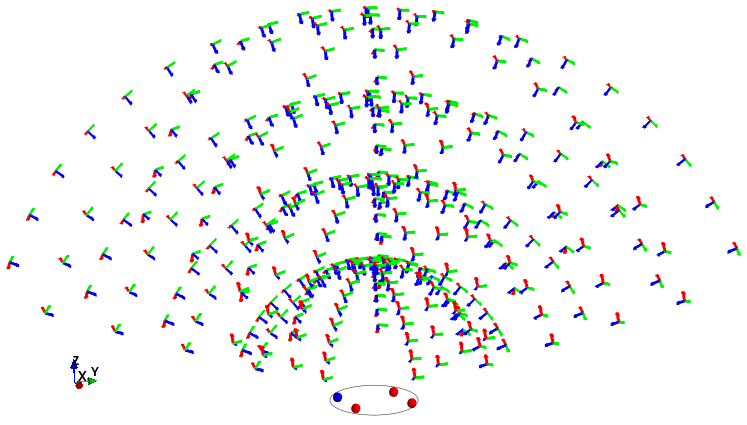
\includegraphics[width=\columnwidth]{img/cam_config3D.png}
			\caption{\label{fig:camera_poses} \small Distribution of 400 camera poses used in simulations. A limiting circular plane with $n$ control points inside is displayed at the bottom. The cameras are distributed evenly on spheres of evenly sampled radii, each one looking at the center of the circular plane. Only camera poses which had all limits of the circular plane in field of view were used.}
		\end{center}
		\vspace{-0.7cm}
	\end{figure}
	
	
	%For each camera pose ${\mathbf{R},\mathbf{t}}$, an initial n-control-points configuration $\{\mathbf{X}^P_{i}\}_{j=0}$ is defined, the variable $j$ represents the iteration number on the gradient descent process. Each initial point of this set is obtained by an uniform-random sampling of the area within the circular plane. Then the gradient descent minimization of \ref{Eq11} is performed for a predefined maximum amount of iterations $j=iters$, obtaining the final optimized point configuration $\{\mathbf{X}^P_{i}\}_{j=iters}$, the intermediate configurations are also saved. So for each camera pose we obtain $\{\mathbf{X}^P_{i}\}_{j}$ with $j \in \{0,iters\}$.
	
	%For the gradient descent minimization of \ref{Eq11} a set of control points and its projections in image coordinates are needed in each iteration. Perfect pairs of correspondences are created for each iteration using the true values of ${\mathbf{R},\mathbf{t}}$ . A more realistic test was also performed using noisy correspondences by adding Gaussian noise to the true values in image coordinates. The results of the gradient descent are similar in both cases, this means that the gradient is mainly driven by the condition number of the $\mathbf{A}$ matrix and not by the noise. Thus, the experiments were performed without noisy correspondences in \ref{Eq11}.
	
	To evaluate the improvement of the gradient descent optimization, 
	we consider the optimization objective, which is the
	condition number \eqref{Eqc} at each iteration $t$, given by $c(\mathbf{A}(t))$ in the DLT algorithm.
	To evaluate the effect of the optimization \eqref{Eq11} on the underlying homography estimate 
	$\hat{\mathbf{H}}(t)$ using a given set of $n$ control points $\{\mathbf{X}^P_{i}\}(t)$,
	we rely on the reprojection error $HE(\hat{\mathbf{H}}(t))$ induced by the estimated homography $\hat{\mathbf{H}}(t)$ given by
	
	\begin{equation}
	HE\left(\hat{\mathbf{H}}(t)\right) = \frac{1}{M}
	\sum\limits_{j=1}^M |\!| \mathbf{x}_j(t) - \pi\left(\hat{\mathbf{H}}(t)\overline{\mathbf{X}}_j^{P}(t)\right)|\!|_2^2\,,
	\end{equation}
	for a fixed set of $M$ validation control points $\{\mathbf{X}_j^{P}\} \not\in \{\mathbf{X}^P_{i}\}(t)$
	that are evenly distributed on the object plane covering an area larger than the limits of the circle.   Thus, it is possible to measure how good $\hat{\mathbf{H}}(t)$ is able to represent the true homography $\mathbf{H}$ beyond the space of the control points.     
	%and $\mathbf{H}$ as the true one for a given camera pose. To evaluate the point configurations obtained by the optimization process two main metrics were considered for the homography estimation:
	
	%\begin{itemize}
	%		\item The condition number \eqref{Eqc} of matrix $\mathbf{A}$ in the DLT algorithm.
	%		\item The reprojection error of the estimated homography $\hat{\mathbf{H}}$ for a set of $M$ validation control points $\{\mathbf{X}_j^{P_v}\}$:
	%\begin{equation}
	%HE(\hat{\mathbf{H}}) = \frac{1}{M}
	%\sum\limits_{j=1}^M |\!| \tilde{\mathbf{x}}_j - \pi(\hat{\mathbf{H}}\overline{\mathbf{X}}_j^{P_v})|\!|_2^2\,.
	%        \end{equation}
	%This validation points are different to the ones used to calculate $\hat{\mathbf{H}}$. Were  $\{\mathbf{X}_j^{P_v}\}$ is a set of $M$ points evenly distributed on the plane $z=0$ covering an area larger than the limits of the circular plane. By using $\{\mathbf{X}_j^{P_v}\}$ 
	%	\end{itemize}
	
	Each simulation for a given camera pose is then performed in the following way: 
	1) An initial random $n$-point set $\{\mathbf{X}^P_{i}\}(t_{start})$ is defined inside the circular plane 
	2) For each iteration step $t$ an improved set of control points $\{\mathbf{X}^P_{i}\}(t)$ is obtained by \eqref{Eq12} and projected to image coordinates $\{\mathbf{x}_{i}\}(t)$ using the true camera pose ${\mathbf{R},\mathbf{T}}$ and calibration matrix $\mathbf{K}$. 
	Then, the correspondences $\{\mathbf{x}_{i}(t), \mathbf{X}^P_{i}(t)\}$ are used to calculate $\mathbf{A}(t)$ and $c(\mathbf{A}(t))$. 
	3) For each $t$ a statistically meaningful measure of the homography estimation robustness against noise is desired. Thus, 1000 runs of the homography estimation using the DLT algorithm were performed\footnote{The homography estimation method presented in \cite{Harker2005} and the gradient based one of OpenCV were also tested. The results almost do not differ for low point configurations to the DLT, so it was the chosen one for the experiments.}. In each of this runs Gaussian noise with standard deviation $\sigma_G$ was added to the image coordinates for the simulation of real camera measurements
	$\{\tilde{\mathbf{x}}_{i}\}(t)$. Finally, the error $HE\left(\hat{\mathbf{H}}(t)\right)$ is calculated in each run and the average $\mu\left(HE\left(\hat{\mathbf{H}}(t)\right)\right)$ and standard deviation $\sigma\left(HE\left(\hat{\mathbf{H}}(t)\right)\right)$ of this error for all runs is computed.% So, for each step $j$ we obtain as result three metrics: $k_2(\mathbf{A})_j$ plus the mean and standard deviation of HE($\hat{\mathbf{H}}_j$).
	
	%NOW WE SHOW SOME RESULTS WITH HOMOGRAPHY
	
	As illustration of the gradient minimization process an example case of a simulation in a fronto-parallel camera pose for a 4-point configuration is presented. A Gaussian noise of $\sigma_G=4$ pixel is added to image coordinates for the homography estimation runs. In Fig. \ref{fig:FP_points} the initial object and image point configurations are shown. The movement of points present two main characteristics: first, they are driven to separate from each other, and second, they tend to equalize distance to each other in object space. This results in stable square-like shaped configurations on average.
	
	%%%%%%%%%%%%%FRONTO PARALLEL CASE
	%245.71811pt
	
	\begin{figure}[t]
		\begin{center}
			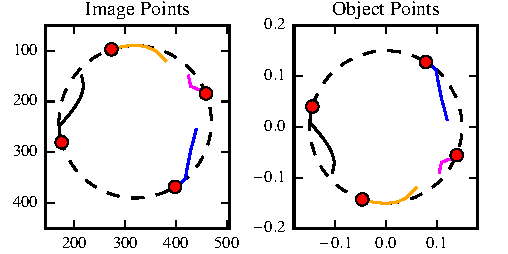
\includegraphics[width=\columnwidth]{img/image_control_points.pdf}
			\caption{\label{fig:FP_points}\small (Fronto-Parallel). Movement of control points (colored lines) in image $\mathbf{x}_i(t)$ and object coordinates $\mathbf{X}^P_i(t)$ during gradient descent optimization for the fronto-parallel camera configuration until the final optimal configuration $\{\mathbf{X}^P_{i}\}(t_{end})$ (red dots) limited by the circle (dotted black line). }
		\end{center}
		\vspace{-0.5cm}
	\end{figure}
	
	%The path followed by each $\mathbf{X}^P_i(t)$ of the minimization process are displayed as coloured lines and the final optimal configuration $\{\mathbf{X}^P_{i}\}(t_{end})$ are filled red dots. The dotted black lines represent the limits of the circular plane.
	
	The evolution of $c(\mathbf{A}(t))$ as well as $\mu\left(HE\left(\hat{\mathbf{H}}(t)\right)\right)$ and $\sigma\left(HE\left(\hat{\mathbf{H}}(t)\right)\right)$
	is presented in Fig. \ref{fig:FP_cond_homo_error}. The condition number decreases drastically in the first iterations of the gradient descent,  and by doing so the mean and standard deviation of $HE\left(\hat{\mathbf{H}}(t)\right)$ is also reduced. With more iterations both metrics slowly and smoothly converge to a minimum stable value. 
	
	\begin{figure}[t]
		\begin{center}
			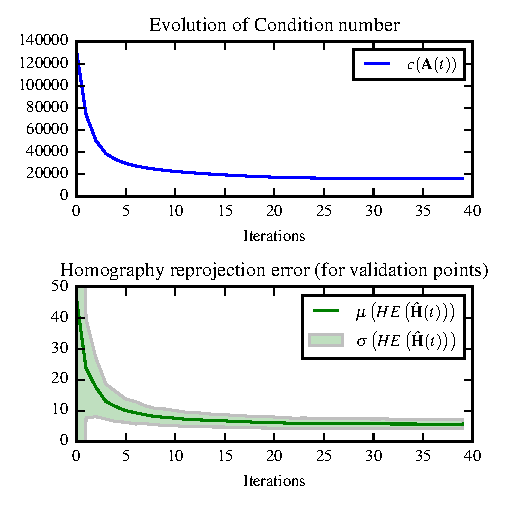
\includegraphics[width=\columnwidth]{img/homography_fronto_parallel.pdf}
			\caption{\label{fig:FP_cond_homo_error}\small(Fronto-Parallel). Evolution of the condition number $c(\mathbf{A}(t))$ as well as mean and standard deviation of the homography reprojection error $HE\left(\hat{\mathbf{H}}(t)\right)$ during gradient descent.}
		\end{center}
		\vspace{-0.0cm}
	\end{figure}
	
	This first result in itself is highly representative as it proves that some point configurations increase the accuracy of homography estimation methods as well as the robustness to noise and it is also possible to obtain optimal point configurations. 
	
	
	%NOW WE SHOW THAT THIS ALSO IMPROVES POSE ESTIMATION
	% DEFINE METRICS
	
	\begin{figure}[t]
		\begin{center}
			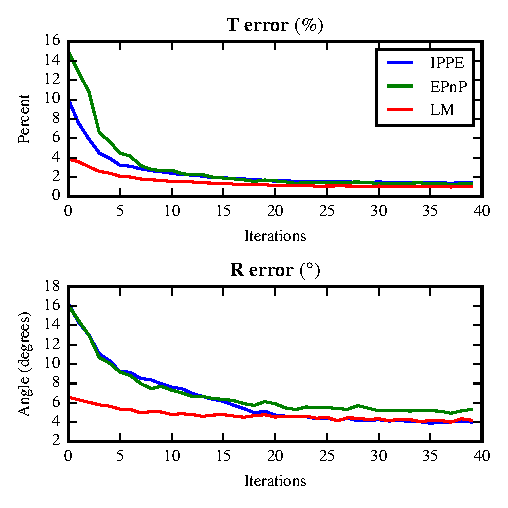
\includegraphics[width=\columnwidth]{img/pose_together_fronto_parallel.pdf}
			\caption{\label{fig:FP_pnp_results_global}\small  (Fronto-Parallel). Comparison of the mean errors for the selected PnP estimation methods during the iterations of the optimization process.}
		\end{center}
		\vspace{-0.5cm}
	\end{figure}
	
	\begin{figure}[t]
		\begin{center}
			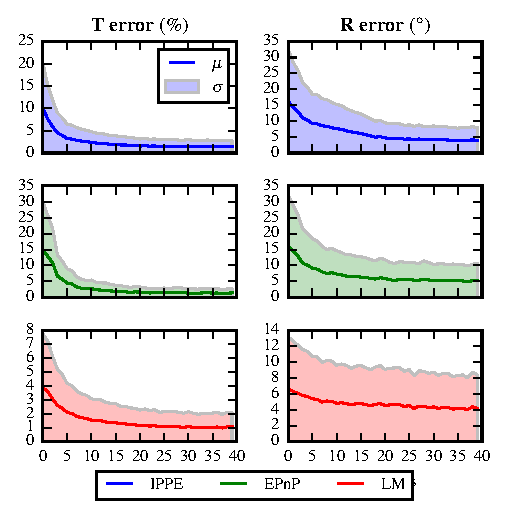
\includegraphics[width=\columnwidth]{img/pose_separate_fronto_parallel.pdf}
			\caption{\label{fig:FP_pnp_results_detailed}\small(Fronto-Parallel). Detailed view of the standard deviation of each method represented by the filled colored areas.}
		\end{center}
		\vspace{-0.5cm}
	\end{figure}
	
	\begin{figure}[t]
		\begin{center}
			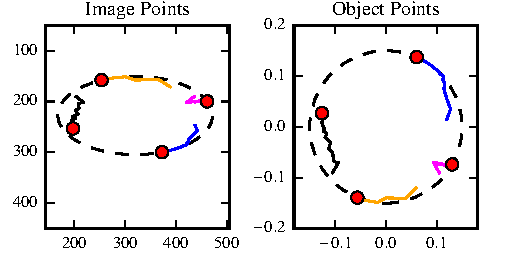
\includegraphics[width=\columnwidth]{img/image_control_points_inclined.pdf}
			\caption{\label{fig:IN_points} \small (Inclined). Movement of control points in image and object coordinates during gradient descent for the inclined camera configuration.}
		\end{center}
		\vspace{-0.5cm}
	\end{figure}
	
	\begin{figure}[t]
		\begin{center}
			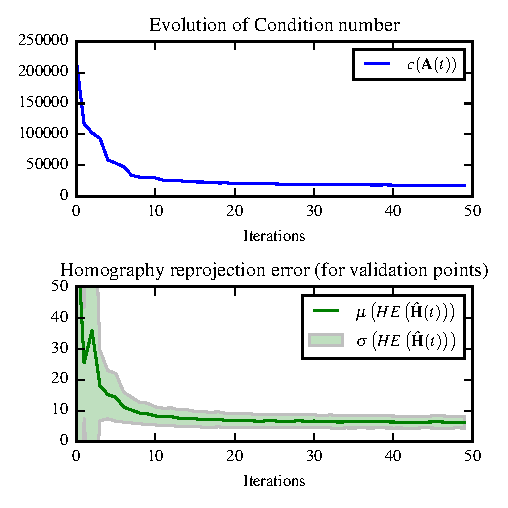
\includegraphics[width=\columnwidth]{img/homography_inclined.pdf}
			\caption{\label{fig:IN_cond_homo_error} \small(Inclined). Evolution of the condition number and the homography reprojection error during gradient descent.}
		\end{center}
		\vspace{-0.5cm}
	\end{figure}
	
	\begin{figure}[t]
		\begin{center}
			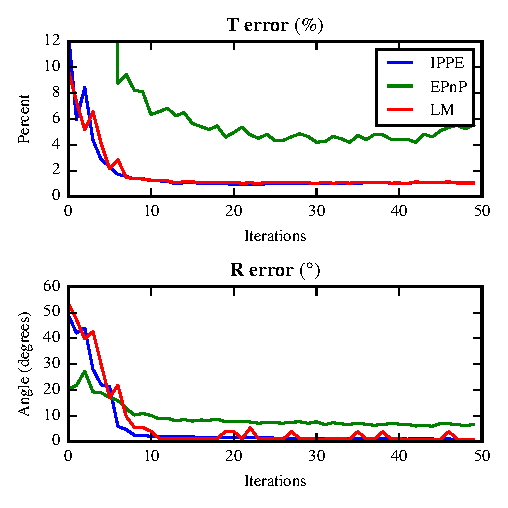
\includegraphics[width=\columnwidth]{img/pose_together_inclined.pdf}
			\caption{\label{fig:IN_pnp_results_global}\small  (Inclined). Comparison of the mean errors for the selected PnP estimation methods during the iterations of the optimization process.}
		\end{center}
		\vspace{-0.5cm}
	\end{figure}
	
	\begin{figure}[t]
		\begin{center}
			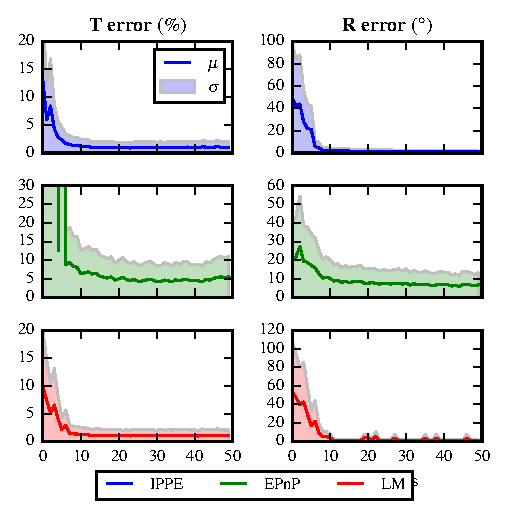
\includegraphics[width=\columnwidth]{img/pose_separate_inclined.pdf}
			\caption{\label{fig:IN_pnp_results_detailed}\small (Inclined). Detailed view of the standard deviation of each method represented by the filled colored areas.}
		\end{center}
		\vspace{-0.5cm}
	\end{figure}
	
	
	
	Motivated by the homography results, it was of interest to test if these point configurations could improve as well the accuracy of pose estimation algorithms. Thus, three different pose estimation algorithms\footnote{For the EPnP and LM methods, the OpenCV implementations were used, and for IPPE the Python implementation provided by the author's github repository.} were run at each iteration $t$ of the optimization process, namely: 1) a non-iterative PnP method \textbf{EPnP}~\cite{Lepetit2008}, 2) a planar pose estimation method \textbf{IPPE}~\cite{Collins2014}, and 3) a fully iterative one based on the Levenberg-Marquardt optimization denoted as \textbf{LM}. 
	
	As in similar works \cite{Lepetit2008,Collins2014}, we denote $\left(\hat{\mathbf{R}}(t), \hat{\mathbf{T}}(t)\right)$ as the estimated rotation and translation for a given camera pose at iteration $t$ and by $(\mathbf{R}, \mathbf{T})$ the true rotation and translation. The error metrics for pose estimation are defined as follows:
	\begin{itemize}
		\item  RE$\left(\hat{\mathbf{R}}(t)\right)$ is the rotational error (in degrees) defined as the minimal rotation needed to align $\hat{\mathbf{R}}(t)$ to $\mathbf{R}$. It is obtained from the axis-angle representation of $\hat{\mathbf{R}}(t)^T\mathbf{R}$.
		
		\item TE$\left(\hat{\mathbf{T}}(t)\right) = \|\hat{\mathbf{T}}(t) - \mathbf{T}\|_2/\|\mathbf{T}\|_2\times 100 \%$ is the relative error in translation. 
	\end{itemize}
	
	%DISCUSS THE RESULTS OF THE POSE
	Similar to the homography simulation, for each iteration $t$, 1000 runs of the pose estimation with noisy correspondences for each of the PnP methods were performed. Then, the mean and standard deviation of RE and TE for the 1000 runs were calculated for each iteration.
	
	The simulation results for the same fronto-parallel example configuration and same initial points of the homography case are presented for the PnP methods in Fig.~\ref{fig:FP_pnp_results_global} and Fig.~\ref{fig:FP_pnp_results_detailed}. For all the compared PnP methods the errors are reduced with iterations. The amount of improvement in EPnP and IPPE is stronger than for LM. The methods converge to similar error values along iterations. As seen in Fig.~\ref{fig:FP_pnp_results_detailed}, not only the mean is reduced but also the variance, with a more pronounced effect on translation for the three methods. It is surprising that the point configuration also affects the performance of LM although our optimization objective is not directly related to the minimization of the reprojection error.
	
	
	
	
	
	
	%PRESENT RESULTS ALSO FOR THE INCLINED AND DISCUSS THEM
	As a comparison, a simulation of an inclined camera pose (30 degrees to the $Z^P=0$ plane) is presented with the same parameters as in the fronto-parallel case. The movements of the control points during the minimization process are presented in Fig. \ref{fig:IN_points}. The condition number and homography estimation error are presented in Fig.~\ref{fig:IN_cond_homo_error}, and the results of the PnP estimation errors are presented in Fig.~\ref{fig:IN_pnp_results_global} and Fig.~\ref{fig:IN_pnp_results_detailed}. As expected, the inclined case presents higher errors on the homography and pose estimation methods. The evolution of the condition number is also less smooth than in the fronto-parallel case which produces some large gradients during optimization and thus spikes in the homography error. This can be removed by finely tuning the SuperSAB parameters of the gradient descent for this particular case but the idea was to compare the simulation with the same parameters of the fronto-parallel case. The EPnP method has a large error with the initial point configuration which improves greatly with the optimization iterations. However, EPnP still has a large final error compared to IPPE and LM. The initial point configuration is also a difficult one for the LM an IPPE method but improves drastically with the optimization.
	
	
	
	%%%%%%%%%%%%%INCLINED CASE
	
	
	
	%EFFECT OF WELL-CONDITIONED VS ILL-CONDITIONED POINT CONFIGURATIONS
	
	
	
	Next, a more profound study was performed. The same steps for simulating a single camera pose as presented in the fronto-parallel and inclined case were used for the total distribution of 400 camera poses shown in Fig. \ref{fig:camera_poses}. For each pose 100 different initial random $n$-point configurations  with $n \in \{4,5,6,7,8\}$ were simulated and the optimization process was performed until finding an optimal point configuration for each. In this case only the initial and final values of the point configuration metrics are stored. Thus, it is possible to compare the methods with 
	\textit{ill-conditioned} (inital points) and \textit{well-conditioned} (after optimization) point configurations.
	
	In Fig.~\ref{fig:comp_homo} the results for the homography estimation are presented and in Fig.~\ref{fig:comp_pose} the results of the pose estimation. The median of the condition number was used instead of the mean since the mean presented high variation due to large particular cases. For the rest of the metrics the mean was selected. 
	It can be seen, that the optimization process finds an optimal point configuration which on average is better for all the camera poses. Further on, the smaller the number of control points the more the optimization of the point configuration improves the homography estimate as well as the pose estimate for all of the evaluated methods. For example, the homography estimate using 4 optimal control points is always better than arbitrary point configurations with more points $4 < n \leq 9$.    
	Choosing more than 4 optimal control points only slightly improves the homography estimates and converges for a number of 8 optimal control points. Thus, configuration of the control points clearly has much more effect on the accuracy than the number of control points. 
	To verify that optimal 4-point configurations with maximal equal distance to each other has the biggest influence on the improvement of accuracy, we performed an additional test: A perfect square inscribed in the limits of the circular plane was selected as initial point configuration for all the camera poses and the metrics were calculated and compared with the results for optimal points obtained from the optimization process. For all of the poses, the square configuration has comparable performance than the optimal point configurations. The reason is because in most of the cases the shape of the final optimization points are also square-like. Thus, we verified that the corners of a square are almost optimal (if not optimal) control point configurations for space resection.
	
	%The homography results show that increasing the number of points reduces the error for ill-conditioned point configurations, however it does not bring much improvements in the well-conditioned case. The tendency of the data indicates that if n is increased an Ill-conditioned configuration may have the same performance than a Well-configured one.%, this validates previous results in the literature about the positive effects of increasing number of control points to overcome noise. The results of the PnP estimation methods also present the same behaviors as the homography which is surprising since the optimization is based only on the condition number of the DLT transform data matrix. 
	
	\begin{figure}[t]
		\begin{center}
			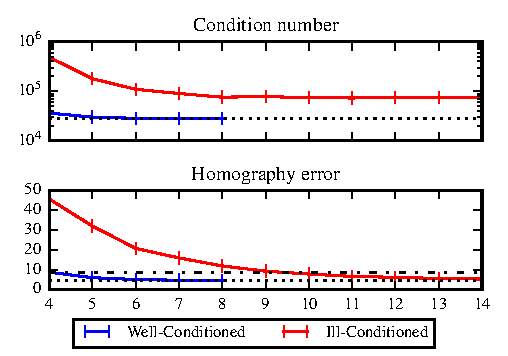
\includegraphics[width=\columnwidth]{img/point_config_comp_homo.pdf}
			\caption{\label{fig:comp_homo}\small Well-conditioned point configurations in contrast to ill-conditioned ones in homography estimation for different numbers of control points.}
		\end{center}
		\vspace{-0.5cm}
	\end{figure}
	
	
	\begin{figure}[t]
		\begin{center}
			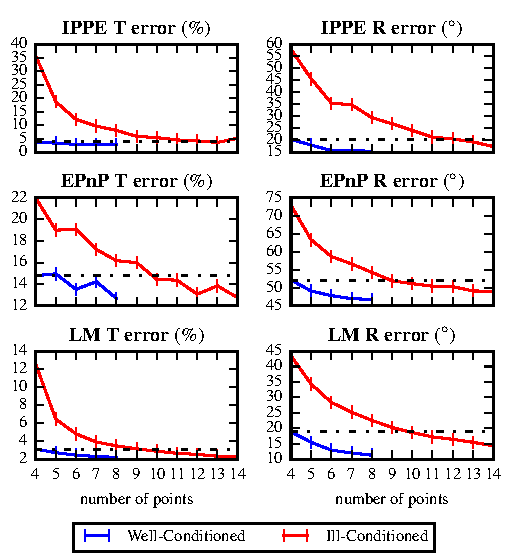
\includegraphics[width=\columnwidth]{img/point_config_comp_pose.pdf}
			\caption{\label{fig:comp_pose}\small Well-conditioned point configurations in contrast to ill-conditioned ones in pose estimation for different numbers of control points.}
		\end{center}
		\vspace{-0.5cm}
	\end{figure}
	
	
	
	\section{Conclusions and future work}
	\label{Conc}
	A method for obtaining optimal control points for homography estimation using an optimization approach is presented. It was shown that for a low amount of control points, the position of the points on the object plane have a strong influence on the accuracy of homography and PnP estimation methods. 
	It was proven that a square is a very stable and robust configuration for all camera poses, which has been a common shape used in planar fiducial markers. For more point configurations the final shapes are not that well defined, however they meet the general rule of being maximally separated in object space with equal distances between each other including the optimal 4-point configuration as a subset. In future work, we will try to generalize the results to non-planar point configurations and head for real dynamic markers that optimize their control points within a visual servoing task. %A first proof of concept can be found in \cite{Acuna17}. 
	%The results of this work are also relevant to fiducial marker designers since they can use the condition number of the DLT data matrix as a metric to evaluate different control point configurations.% Finally we believe that in cases were a large number of points are obtained by a feature matching process (e.g SURF) the results presented in this paper can be used to select a subgroup of points which are well-conditioned and then reduce computation time of pose estimation methods by using less points.
	
	%\addtolength{\textheight}{-12cm}   % This command serves to balance the column lengths
	% on the last page of the document manually. It shortens
	% the textheight of the last page by a suitable amount.
	% This command does not take effect until the next page
	% so it should come on the page before the last. Make
	% sure that you do not shorten the textheight too much.
	
	%%%%%%%%%%%%%%%%%%%%%%%%%%%%%%%%%%%%%%%%%%%%%%%%%%%%%%%%%%%%%%%%%%%%%%%%%%%%%%%%
	
	
	
	%%%%%%%%%%%%%%%%%%%%%%%%%%%%%%%%%%%%%%%%%%%%%%%%%%%%%%%%%%%%%%%%%%%%%%%%%%%%%%%%
	
	
	
	%%%%%%%%%%%%%%%%%%%%%%%%%%%%%%%%%%%%%%%%%%%%%%%%%%%%%%%%%%%%%%%%%%%%%%%%%%%%%%%%
	%%%%%%%%%%%%%%%%%%%%%%%%%%%%%%%%%%%%%%%%%%%%%%%%%%%%%%%%%%%%%%%%%%%%%%%%%%%%%%%%
	%\section*{Acknowledgements}
	
	{\small
		\bibliography{IEEEabrv,bib_icra2018,volker}
		
		
		
	}
\end{document}


